\documentclass[12pt]{article}

% \graphicspath{Figures/}  % Location of the graphics files (set up for graphics to be in PDF format)
\usepackage{float}
\usepackage{amsmath}
\usepackage{multirow}
\usepackage{xcolor}
\usepackage{lipsum}
\usepackage{siunitx}
\usepackage{physics}
\usepackage{graphicx}
\usepackage{mathrsfs}
\usepackage{verbatim}  % Needed for the "comment" environment to make LaTeX comments

%% ------------------ tikz ---------------------------------------
\usepackage{pgfplots}
\usepackage{tikz}
\usepackage{tikz-layers}
\usetikzlibrary{shapes.geometric, arrows,cd}
\tikzstyle{startstop} = [rectangle, rounded corners, minimum width=3cm, minimum height=1cm, text centered, draw=black, fill=white]
\tikzstyle{arrow1}=[ultra thick,->,>=stealth]
\tikzstyle{arrow}=[thick,->,>=stealth]
\tikzset{
  shift left/.style ={commutative diagrams/shift left={#1}},
  shift right/.style={commutative diagrams/shift right={#1}}
}
\pgfplotsset{compat=1.17}

\begin{document}

\newcommand\gauss[2]{1/(#2*sqrt(2*pi))*exp(-((x-#1)^2)/(2*#2^2))} % Gauss function, parameters mu and sigma
\usepgfplotslibrary{fillbetween}
\usetikzlibrary{positioning}
\usetikzlibrary{shapes.multipart}
\usetikzlibrary{arrows,calc,fit}
\usetikzlibrary{matrix,backgrounds,decorations.pathreplacing,positioning}

\begin{figure}
        \centering
        \begin{tikzpicture}[every text node part/.style={align=center}]
            
            % draw a background box for the density overlap and the two gaussian curves
            \node[rectangle, very thick,dashed,draw=black,fill=none] (huge-container-box) [minimum height=5cm,minimum width=12cm,xshift=0.7cm,yshift=-0.3cm] at (2,2.5) {};
            
            \begin{scope}[xshift=1cm]
                % add coupling schematic
                \draw[-latex] [thick, color=black,dashed] (1.5,6) -- (6,6) node [yshift=-0.3cm] {$m$-axis};
                \draw[-latex] [thick, color=black,dashed] (1.5,6) -- (6,6) node [yshift=+0.4cm,xshift=0.3cm] {$\mathcal{I}_m$ - largest MOI};
                \draw[-latex] [thick, color=black,dashed] (1.5,6) -- (1.5,9) node [pos=1,above] {$s$-axis};
                \draw[-latex] [ultra thick, color=black!60!green] (1.5,6) -- (4,6) node [yshift=0.4cm] {$\mathbf{j}_{\mathscr{C}}$};
                \draw[-latex] [ultra thick, color=magenta] (1.5,6) -- (1.5,8) node [xshift=-0.5cm] (my-arrow) {$\mathbf{j}_{\mathcal{Q}_p}$};
                % \draw[-latex] [ultra thick, color=magenta] (1.5,6) -- (1.5,8) node [pos=1,above,xshift=-1cm] (my-arrow) {$\mathbf{j}_{\mathcal{Q}_p}$};
                \node[rectangle, draw=black, fill=none,anchor=south west] at (1.5,6) {};
                \node[rectangle, draw=black, fill=green!10,anchor=south west, minimum width=4cm] at (3,7.5) (coupling-box) {$(\mathcal{Q}_p+\mathscr{C})$\\ Coupling};
            \end{scope}
            
            \node[rectangle, draw=black, thick, fill=green!10, inner sep=0.2cm,minimum width=12 cm] at (2,-1.8) (first-box) {\textbf{Minimized} short-range interaction \\ \\ $\mathcal{Q}_p+\mathscr{C}$ = \emph{attractive}};
            
            \node[rectangle, draw=black, thick, fill=green!10, inner sep=0.2cm,minimum width=12 cm] (second-box) [below=of first-box] {\textbf{Minimal} energy (PES)};
            
            \node[rectangle, draw=black, thick, fill=green!10, inner sep=0.2cm,minimum width=12 cm] (third-box) [below=of second-box] {\textbf{Stable triaxial shape} \\ $\downarrow$ \\ \textbf{Transverse Wobbling Motion}: $\mathbf{j}_{\mathcal{Q}_p}\perp (m_\text{axis}\ ||\  \mathbf{j}_\mathscr{C})$};

            \node[rectangle, draw=black,xshift=6cm,yshift=2cm,fill=green!10, minimum width=4cm] (maximal-box) {\textbf{Maximal overlap} \\ between \\ {\color{magenta}$\mathcal{D}\left(\mathcal{Q}_p\right)$} and {\color{black!60!green}$\mathcal{D}\left(\mathscr{C}\right)$}};


            % \draw[-latex] [very thick,black] (inside-node.east) -- ($(inside-node.east)+(2.2,0)$) |- node [xshift=-1.9cm,yshift=2.7cm] (maximal-box) {\textbf{Maximal overlap} \\ between \\ {\color{magenta}$\mathcal{D}\left(\mathcal{Q}_p\right)$} and {\color{black!60!green}$\mathcal{D}\left(\mathscr{C}\right)$}} (first-box.east);
            % \draw[-latex] [very thick,black] (first-box) -- node[circle,draw=black,xshift=1cm] {a} (second-box);
            \draw[-latex] [very thick,black] (first-box) -- node[circle,draw=black,xshift=1cm,fill=yellow!30] {$4$} (second-box);
            \draw[-latex] [very thick,black] (second-box) -- node[circle,draw=black,xshift=1cm,fill=yellow!30] {$5$} (third-box);
            % \draw[-latex] [very thick, color=black] (1.5,5.5) -| (maximal-box.east);
            
            % draw arrow for coupling and maximal overlap
            \draw[-latex] [very thick, color=black] (coupling-box.east) -- ($(coupling-box.east)+(1,0)$) |- node[circle,draw=black,xshift=-0.4cm,yshift=-0.6cm,fill=yellow!30] {$2$} (maximal-box.east);

            \begin{axis}[scale=0.6,xshift=-2cm,every axis plot post/.append style={
                mark=none,domain=-2:3,samples=50,smooth}, % All plots: from -2:2, 50 samples, smooth, no marks
                axis x line*=bottom, % no box around the plot, only x and y axis
                axis y line*=left, % the * suppresses the arrow tips
                axis line style={draw=none},
                xtick=\empty, ytick=\empty,
                enlargelimits=false, 
                clip=false, 
                axis on top,
                grid = major,
                legend style={at={(1,1)},anchor=north,legend cell align=left}
                ]
                % extend the axes a bit to the right and top
                
                \addplot [name path=particle-density, color=magenta,very thick] {\gauss{0}{0.5}};
                \addplot [name path=core-density, color=black!60!green,very thick] {\gauss{0.5}{0.65}};
                \legend{$\mathcal{D}\left(\mathcal{Q}_p\right)$,$\mathcal{D}\left(\mathscr{C}\right)$}
                \path[name path=axis] (axis cs:1,0) -- (axis cs:2,0);
                
                % path for fixing boundaries which will be used to fill common region between gaussian curves
                \path[name path=lower,intersection segments={of=particle-density and core-density, sequence={L1 -- R2 -- L3}}];
                
                \node[rectangle, draw=none, thick, fill=none] at (axis cs: 0.8,0.9) (inside-node) {Density distributions for $\mathcal{Q}_p$ and $\mathscr{C}$};
                
                \addplot[color=gray!30] fill between[of= lower and axis];
            \end{axis}

            \begin{scope}[yshift=6cm,xshift=-4cm]
                % draw Fermi orbital for a j-particle
                \node[rectangle, very thick,draw=black,fill=yellow!50] (jshell-box) [minimum height=3cm,minimum width=2cm] at (2.5,1.5) {};
                \foreach \x [count=\xi] in {0.1,0.2,0.3,0.4,0.5,0.6} { 
                    \draw (2,\xi em) -- (3,\xi em) ;
                }
                \node at (1.8,0.4) {$\mathcal{Q}_p$};
                \node[circle,draw=none,fill=magenta] at (2.5,0.4) {};
                \node[] at (2.5,-0.5) {$j$-shell};
            \end{scope}

            %draw arrow from jshell to coupling box
            \draw[-latex,very thick] (jshell-box.north) -- ($(jshell-box.north)+(0,1cm)$) node[circle,draw=black,yshift=-0.6cm,xshift=8.1cm,fill=yellow!30] {$1$} -| (coupling-box);

            % connect maximal overlap with minimal interaction
            \draw[-latex,very thick] (maximal-box.south) -- ($(maximal-box.south)-(0,0.4cm)$) -| node[draw=black,circle,yshift=-0.5cm,xshift=0.6cm,fill=yellow!30] {$3$} ([xshift=1cm]first-box.north);
        
        \end{tikzpicture}
        
        \caption{The workflow of a quasi-particle with particle character $\mathcal{Q}_p$ in its coupling with a triaxial rotor $\mathscr{C}$. Each of the five `steps' represents a characteristic involved in the wobbling motion, as described in text. Namely, for $\mathcal{Q}_p$ coming from the bottom of a $j$-shell and coupling with the $s$-axis of the even-even core $\mathscr{C}$ \textbf{(1)} will maximize the density overlap \textbf{(2)}, which will minimize their interaction \textbf{(3)}, minimizing the total energy \textbf{(4)}, and finally stabilizing the triaxial structure \textbf{5}. The long $l$-axis has been ignored within the drawings.}
        \label{advanced-quasiparticle-coupling-1}
\end{figure}


\begin{figure}
    \centering
    \begin{tikzpicture}[every text node part/.style={align=center}]
        
        % draw a background box for the density overlap and the two gaussian curves
        \node[rectangle, very thick,dashed,draw=black,fill=none] (huge-container-box) [minimum height=5cm,minimum width=12cm,xshift=0.7cm,yshift=-0.3cm] at (2,2.5) {};
        
        \begin{scope}[xshift=1cm]
            % add coupling schematic
            \draw[-latex] [thick, color=black,dashed] (1.5,6) -- (6,6) node [yshift=-0.3cm] {$m$-axis};
            \draw[-latex] [thick, color=black,dashed] (1.5,6) -- (6,6) node [yshift=+0.4cm,xshift=0.3cm] {$\mathcal{I}_m$ - largest MOI};
            \draw[-latex] [thick, color=black,dashed] (1.5,6) -- (1.5,9) node [pos=1,above] {$l$-axis};
            \draw[-latex] [ultra thick, color=black!60!green] (1.5,6) -- (4,6) node [yshift=0.4cm] {$\mathbf{j}_{\mathscr{C}}$};
            \draw[-latex] [ultra thick, color=blue] (1.5,6) -- (1.5,8) node [xshift=-0.5cm] (my-arrow) {$\mathbf{j}_{\mathcal{Q}_n}$};
            % \draw[-latex] [ultra thick, color=magenta] (1.5,6) -- (1.5,8) node [pos=1,above,xshift=-1cm] (my-arrow) {$\mathbf{j}_{\mathcal{Q}_p}$};
            \node[rectangle, draw=black, fill=none,anchor=south west] at (1.5,6) {};
            \node[rectangle, draw=black, fill=red!10,anchor=south west, minimum width=4cm] at (3,7.5) (coupling-box) {$(\mathcal{Q}_n+\mathscr{C})$\\ Coupling};
        \end{scope}
        
        \node[rectangle, draw=black, thick, fill=red!10, inner sep=0.2cm,minimum width=8 cm] at (2,-1.8) (first-box) {\textbf{Minimized} short-range interaction \\ \\ $(\mathcal{Q}_n+\mathscr{C})$ = \emph{repulsive}};
        \node[rectangle] (pes-image-box) [right=of first-box,xshift=-0.7cm] {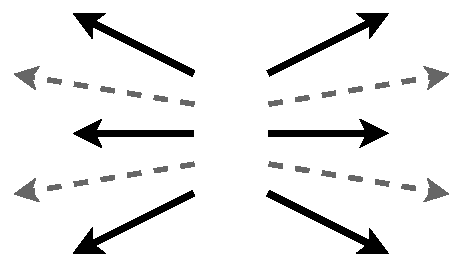
\includegraphics[scale=0.3]{Chapters/Figures/repulsive_interaction.pdf}};
        
        \node[rectangle, draw=black, thick, fill=red!10, inner sep=0.2cm,minimum width=8 cm] (second-box) [below=of first-box] {\textbf{Minimal} energy (PES)};
        \node[rectangle] (pes-image-box) [right=of second-box,xshift=-0.7cm,yshift=0.4cm] {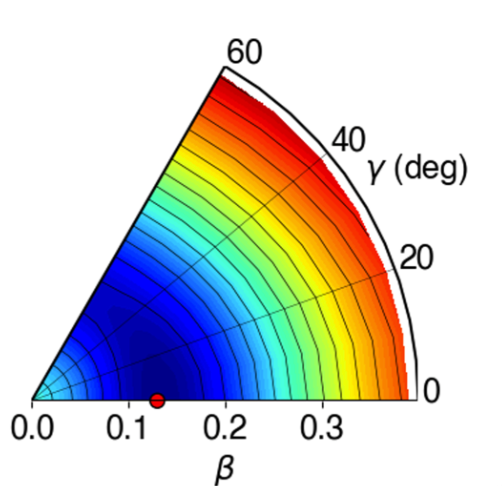
\includegraphics[scale=0.12]{Chapters/Figures/PES_small_update.png}};
        
        \node[rectangle, draw=black, thick, fill=red!10, inner sep=0.2cm,minimum width=8 cm] (third-box) [below=of second-box] {\textbf{Stable triaxial shape} \\ $\downarrow$ \\ \textbf{Transverse Wobbling Motion}: \\ $\mathbf{j}_{\mathcal{Q}_n}\perp (m_\text{axis}\ ||\  \mathbf{j}_\mathscr{C})$};
        \node[rectangle] (precession-cone-box) [right=of third-box,xshift=-1cm] {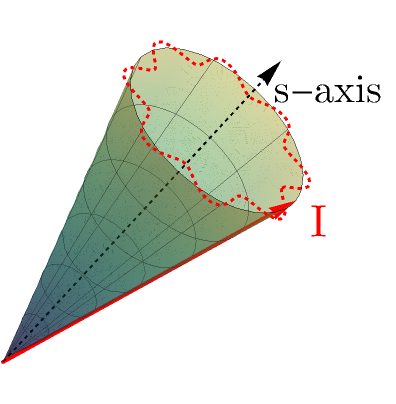
\includegraphics[scale=0.25]{Chapters/Figures/precessional_cone.png}};
        
        \node[rectangle, draw=black,xshift=6cm,yshift=2cm,fill=red!10, minimum width=4cm] (maximal-box) {\textbf{Minimal overlap} \\ between \\ {\color{blue}$\mathcal{D}\left(\mathcal{Q}_n\right)$} and {\color{black!60!green}$\mathcal{D}\left(\mathscr{C}\right)$}};


        % \draw[-latex] [very thick,black] (inside-node.east) -- ($(inside-node.east)+(2.2,0)$) |- node [xshift=-1.9cm,yshift=2.7cm] (maximal-box) {\textbf{Maximal overlap} \\ between \\ {\color{magenta}$\mathcal{D}\left(\mathcal{Q}_p\right)$} and {\color{black!60!green}$\mathcal{D}\left(\mathscr{C}\right)$}} (first-box.east);
        % \draw[-latex] [very thick,black] (first-box) -- node[circle,draw=black,xshift=1cm] {a} (second-box);
        \draw[-latex] [very thick,black] (first-box) -- node[circle,draw=black,xshift=1cm,fill=yellow!30] {$4$} (second-box);
        \draw[-latex] [very thick,black] (second-box) -- node[circle,draw=black,xshift=1cm,fill=yellow!30] {$5$} (third-box);
        % \draw[-latex] [very thick, color=black] (1.5,5.5) -| (maximal-box.east);
        
        % draw arrow for coupling and maximal overlap
        \draw[-latex] [very thick, color=black] (coupling-box.east) -- ($(coupling-box.east)+(1,0)$) |- node[circle,draw=black,xshift=-0.4cm,yshift=-0.6cm,fill=yellow!30] {$2$} (maximal-box.east);

        \begin{axis}[scale=0.6,xshift=-2cm,every axis plot post/.append style={
            mark=none,domain=-2:3,samples=50,smooth}, % All plots: from -2:2, 50 samples, smooth, no marks
            axis x line*=bottom, % no box around the plot, only x and y axis
            axis y line*=left, % the * suppresses the arrow tips
            axis line style={draw=none},
            xtick=\empty, ytick=\empty,
            enlargelimits=false, 
            clip=false, 
            axis on top,
            grid = major,
            legend style={at={(1,1)},anchor=north,legend cell align=left}
            ]
            % extend the axes a bit to the right and top
            
            \addplot [name path=particle-density, color=blue,very thick] {\gauss{0}{0.5}};
            \addplot [name path=core-density, color=black!60!green,very thick] {\gauss{0.5}{0.65}};
            \legend{$\mathcal{D}\left(\mathcal{Q}_n\right)$,$\mathcal{D}\left(\mathscr{C}\right)$}
            \path[name path=axis] (axis cs:1,0) -- (axis cs:2,0);
            
            % path for fixing boundaries which will be used to fill common region between gaussian curves
            \path[name path=lower,intersection segments={of=particle-density and core-density, sequence={L1 -- R2 -- L3}}];
            
            \node[rectangle, draw=none, thick, fill=none] at (axis cs: 0.8,0.9) (inside-node) {Density distributions for $\mathcal{Q}_n$ and $\mathscr{C}$};
            
            \addplot[color=gray!30] fill between[of= lower and axis];
        \end{axis}

        \begin{scope}[yshift=6cm,xshift=-4cm]
            % draw Fermi orbital for a j-particle
            \node[rectangle, very thick,draw=black,fill=yellow!50] (jshell-box) [minimum height=3cm,minimum width=2cm] at (2.5,1.5) {};
            \foreach \x [count=\xi] in {0.1,0.2,0.3,0.4,0.5,0.6} { 
                \draw (2,\xi em) -- (3,\xi em) ;
            }
            \node at (1.8,2.5) {$\mathcal{Q}_n$};
            \node[circle,draw=none,fill=blue] at (2.5,2.5) {};
            \node[] at (2.5,-0.5) {$j$-shell};
        \end{scope}

        %draw arrow from jshell to coupling box
        \draw[-latex,very thick] (jshell-box.north) -- ($(jshell-box.north)+(0,1cm)$) node[circle,draw=black,yshift=-0.6cm,xshift=8.1cm,fill=yellow!30] {$1$} -| (coupling-box);

        % connect maximal overlap with minimal interaction
        \draw[-latex,very thick] (maximal-box.south) -- ($(maximal-box.south)-(0,0.4cm)$) -| node[draw=black,circle,yshift=-0.5cm,xshift=0.6cm,fill=yellow!30] {$3$} ([xshift=1cm]first-box.north);
    
    \end{tikzpicture}
    
    \caption{The workflow of a quasi-particle with hole character $\mathcal{Q}_n$ in its coupling with a triaxial rotor $\mathscr{C}$. Each of the five `steps' represents a characteristic involved in the wobbling motion, as described in text. Namely, for $\mathcal{Q}_n$ coming from the top of a $j$-shell and coupling with the $l$-axis of the even-even core $\mathscr{C}$ \textbf{(1)} will minimize the density overlap \textbf{(2)}, which will minimize their interaction \textbf{(3)}, minimizing the total energy \textbf{(4)}, and finally stabilizing the triaxial structure \textbf{5}. The short $s$-axis has been ignored within the drawings.}
    \label{advanced-quasiparticle-coupling-2}
\end{figure}

\end{document}
